\chapter{Dispositivos}

\section{GPS}

O sistema GPS oferece aos usuários, informação exata, continua e tridimensional de posição e velocidade de maneira ilimitada, uma vez que os usuários atuam de forma passiva. Para determinar a posição do usuário, o sistema utiliza o conceito one-way time arrivel, TOA, que mede o tempo que o sinal transmitido por um emissor em um local conhecido, leva para chegar ao receptor, multiplica o de tempo pela velocidade de propagação do sinal e assim obtém a distância emissor-receptor. 

Tendo em vista que o sistema proposto com este projeto visa calcular e identificar quando há ou não a possibilidade de ultrapassagem, o sistema GPS é necessário para identificar a posição dos veículos quando há a intenção de ultrapassagem, já que, como citado anteriormente, em qualquer ponto da terra, pelo menos 4 satélites conseguem identificar a posição do usuário, além disso não há necessidade de intervisibilidade entre estações para seu funcionamento e ele opera sob quaisquer condições climáticas.

O sistema receptor armazena o tempo medido e os valores de tempo registrados pelos satélites no momento do envio da onda portadora, com base nesse dado e na velocidade de propagação das ondas, que é conhecida, através da equação (1) se obtém a distância \cite{8gps}.

 $ \Delta S = V \times  \Delta t $

 Onde:

 $ \Delta S $ é a distância entre o satélite e o receptor.
V é a velocidade de propagação da onda.

$ \Delta t $ é o tempo de envio da onda portadora.

O GPS possui três segmentos, espacial, de controle e de usuário, a figura \ref{fig:segmentos_gps} ilustra a iteração dos segmentos.

Dentro do CIAC, os módulos de GPS, indicaram a posição e a velocidade, tanto do carro que vai ultrapassar, quanto do carro a ser ultrapassado e do carro vindo em direção contrária.

\begin{figure}[h]
  \centering
  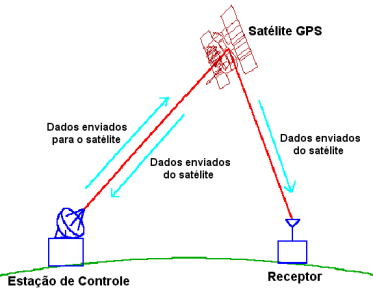
\includegraphics[width=350px, scale=1]{figuras/segmentos_gps}
  \caption{Segmentos de GPS  \cite{9gps}}
\label{fig:segmentos_gps}
\end{figure}

\subsection{Escolha}

Foi constatado que os GPS têm valores de restrição muito parecidos, além de estarem na mesma faixa de preço. Dessa forma o fator decisivo para a escolha do módulo foi a interface serial. Conforme as especificações do Transponder a ser utilizado no projeto, o módulo de GPS escolhido foi o ME-1000RW, que tem a mesma interface serial que o dispositivo. Como módulo secundário, foi escolhido o A2200-A, que tem fabricante e funcionamento diferente do primeiro módulo, para dar mais segurança e redundância ao projeto.

\section {Tela de Interface}

Interface é o nome dado a toda a porção de um sistema com a qual um usuário mantém contato ao utilizá-lo, tanto ativa quanto passivamente, engloba tanto software quanto hardware.

Para atender às necessidades deste projeto, a interface deve fazer comunicação apenas do sistema para o usuário, de modo a deixar o sistema o mais autônomo possível.

Por meio das pesquisas, foi constatado que as telas têm valores de restrição muito parecidos, além de estarem na mesma faixa de preço. Dessa forma, a tela escolhida foi a TFT054A, porque, além de ter um menor preço em relação a TFT052A, tem mais aplicabilidades em relação as duas outras telas citadas.

\section{Sensor de Rotação}

Para fins de projeto, foi necessário que se escolhesse alguns sensores o qual possibilitasse que o sistema de alerta anti-colisão identificasse quando o motorista apresenta intenção de ultrapassagem, para esse fim, foi escolhido um sensor de rotação o qual identifica a posição angular da direção do veículo, onde ao girar o volante no sentido da ultrapassagem, o sensor calcula a angulação de giro enviando esses dados para o microprocessador onde será processado todas as ações do sistema.

O novo PST-360 Piher apresenta uma tecnologia exclusiva sem contato que detecta a posição dos eixos mais de 360 graus com precisão até 0,5\%. Este dispositivo pode ser programado com saída de escala completa durante ângulos menores. A saída é selecionável entre Analógica, PWM e SPI. Além disso, a tecnologia da Piher mantém a sua posição , mesmo depois de uma interrupção de energia.

Um dos motivos pelo qual o sensor PST-360 foi escolhido é que o mesmo oferece o suporte de encaixe diretamente no eixo de direção do volante, permitindo assim, que não seja necessário existir nenhum suporte adicional na sua instalação. As especificações do mesmo podem ser encontradas nos apêndices.

\begin{figure}[h]
  \centering
  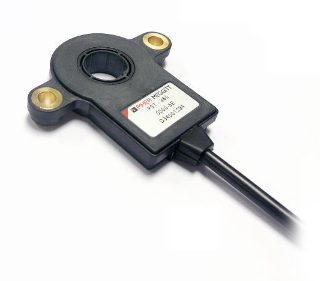
\includegraphics[width=350px, scale=1]{figuras/pst}
  \caption{Sensor de rotação PST-360}
\label{fig:pst}
\end{figure}


\section{Câmera}

Para uma melhor análise das condições de tráfego veicular nas rodovias, com o intuito de projetar um sistema que emite alertas de colisão veicular, fez-se necessário o acréscimo de uma câmera a qual possibilitasse colher mais informações do tráfego dos veículos, assim como sua posição na pista, com objetivo de diminuir os erros de dados do sistema. Para isso foi escolhido uma câmera com base no sistema anti colisão  Toyota Safety Sense , cujo modelo é o AWS650 da 3M.

Dentro do Sistema, câmera atuará de forma a identificar a mudança de faixa, a velocidade do veículo da frente e mostrar as imagens da pista, tanto à noite, quanto durante o dia.

\subsection{Escolha}

Com base nos requisitos do projeto, foi escolhido a câmera AWS650, pois a mesma atende todos os requisitos do projeto na qual será utilizado todas as funções da câmera. Tal escolha foi baseada no sistema da Toyota Safety Sense, em que não foi escolhido por possuir excesso de funções que não vão ser úteis para o sistema, além de tais funções interferirem no funcionamento do veiculo, como o acionamento dos freios  por exemplo,  onde viola a restrição do projeto no qual diz que o sistema não pode interferir nas funções de funcionamento do veículo.

O sistema AWS apenas tem a função de alertar a segurança ao condutor, cabendo a ele tomar as devidas ações necessárias para corrigir o veículo de forma a manter a segurança, aspecto esse, que atende ao requisito do projeto de não alterar as funções do veículo, apenas oferecer ao condutor a informação.
	
Para um melhor funcionamento em modo noturno foi necessário fazer uma adaptação na câmera, tal modificação encontra-se nos apêndices.

\begin{figure}[h]
  \centering
  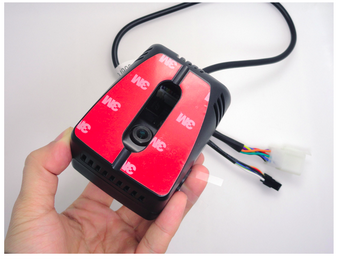
\includegraphics[width=350px, scale=1]{figuras/sensoraws650}
  \caption{Dispositivo AWS650}
\label{fig:sensoraws650}
\end{figure}

\section{LIDAR}

O Lidar é uma tecnologia de detecção usado para medição de distâncias ou outras informações relevantes. No CIAC, o Lidar funcionará de forma a identificar a velocidade e a posição dos veículos envolvidos na ultrapassagem.

\begin{figure}[h]
  \centering
  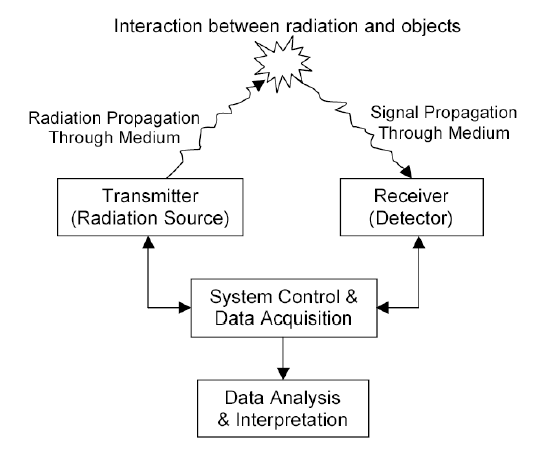
\includegraphics[width=350px, scale=1]{figuras/funcionamento_lidar}
  \caption{Esquemático do funcionamento do Lidar}
\label{fig:funcionamento_lidar}
\end{figure}


\subsection{Escolha}

O Lidar será utilizado no CIAC para medição de diversas distâncias entre carros, sendo eles os que estão sendo ultrapassados ou os que estiverem na via oposta durante a ultrapassagem.

A detecção de luz e o mapeamento com o Lidar é um método preciso para medição de referências espaciais e distâncias de objetos, além de fazer uma varredura para obtenção dos dados não sendo um detector pontual. O Lidar servirá como um sensor para uma maior confiabilidade do sistema CIAC e permite a obtenção de dados a partir de ondas eletromagnéticas (o processo físico é extremamente rápido) fazendo com que a demora para obtenção da distância entre um carro e outro dependa em sua maior parte apenas do processamento desses dados. Uma grande precisão em um pequeno intervalo de tempo faz do Lidar uma boa opção na utilização do projeto. Todas as especificações podem ser encontradas nos apêndices.

\section{Radar}

O radar é um dispositivo amplamente utilizado que possui grande confiabilidade. Várias empresas automotivas utilizam de radares para detecção de distâncias e velocidades já que se pode ter uma medição precisa e as interferências causadas pelo ambiente ou por condições climáticas poderem, algumas vezes, ser contornados. O Radar funcionará de forma a identificar a posição e a velocidade dos veículos envolvidos na ultrapassagem.

\section{Laser para a Câmera}

Segundo Marco Aurélio, O raio laser é um tipo de radiação eletromagnética visível ao olho humano. A luz do laser além de ser monocromática, ou seja, constituída por radiações de uma única frequência, é muito potente em razão da grande concentração de energia em pequenas áreas (pequenos feixes). O feixe de laser é muito potente, podendo ter brilho superior ao da luz emitida por uma lâmpada.

No sistema, o laser será acrescentado à câmera, de forma a adaptar a mesma para um funcionamento adequado durante a noite.

\subsection{Escolha}

Fez-se necessário a escolha de um laser a fim de auxiliar na adaptação da câmera usada no projeto, a AWS650, no qual irá auxiliá-la no funcionamento noturno. A AWS650 possui também funcionamento noturno, porém, com o incremento do laser, irá assim aumentar o raio de alcance da mesma. 

Segundo o Manual do usuário do Laser Nano Series, um sistema de feedback negativo garante que o raio laser ponha para fora exatamente a mesma quantidade de feixes de luz a partir do momento que o liga até o último segundo do poder da bateria.

Dessa forma, o laser utilizado será o Nano Series da empresa Wicked Lasers, que possui um alcance de 141 metros, distância esta sendo mais que suficiente para a adaptação da câmera no funcionamento noturno, fazendo dessa forma com que haja melhoria no alcance de imagens em situações de escuridão acentuada onde apenas as configurações da câmera não funcionaria .

\begin{figure}[h]
  \centering
  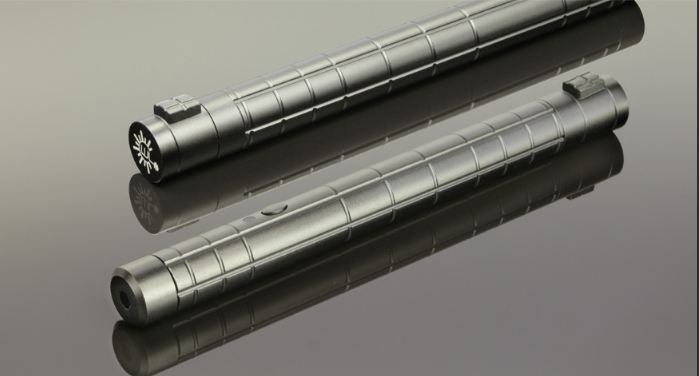
\includegraphics[width=350px, scale=1]{figuras/laser_nano}
  \caption{Laser Nano Series da Wicked Lasers}
\label{fig:laser_nano}
\end{figure}

\section{Microprocessador}

ARM é uma arquitetura de processadores que é largamente usado em sistemas embarcados por possuir instruções simplificadas e a filosofia de obtenção de máxima performance por ciclo e ter um baixo consumo. A linha de processadores ARM Cortex -A8 é uma linha de processadores que utilizam o conjunto de instruções ARMv7 e tem como objetivo o baixo consumo e a alta performance.

\begin{figure}[h]
  \centering
  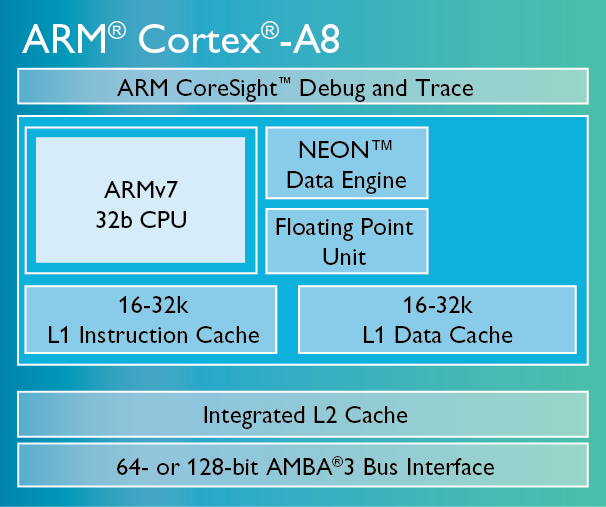
\includegraphics[width=350px, scale=1]{figuras/arm}
  \caption{Diagrama de um processador Arm}
\label{fig:arm}
\end{figure}

Mas como o consórcio ARM não produz esse tipo de processador, utilizaremos a linha AM335x fabricado pela texas instrument. Essa linha é um System on a Chip (Sitema em um Chip ou SoC) onde em um chip possui todas as especificações de um sistema completo, com possibilidade de escrever um sistema operacional básico em suam memória flash.

Além de tudo o processador AM335x possui blocos de tratamento próprio para imagem, para display e principalmente 69 saídas do tipo GPIO (General Propouse Input e Output ou Saídas e entradas de propósito geral) sendo 10 dessas saídas analógicas. Ele tem clock interno de 1Ghz e memória interna de 512 MiB.

\section{Transponder VDL 4000/VTE CNS SYSTEMS}

\subsection{Funcionamento}

Transponder é a abreviatura para transmiter/responder, ou seja, um sistema composto de um leitor, que solicita os dados armazenados em um segundo transmissor, ou seja, um sistema de comunicação em duas vias.

Como referência, já existe um sistema de transponders homologado para identificação veicular em rodovias no Brasil, o SINIAV, que tem o intuito de identificar os veículos que trafegam pelas rodovias ao passarem por postos de controle espalhados ao longo do trajeto. Uma aplicação mais rotineira de uma espécie de transponder é o sistema de pagamento automático de pedágios em estradas sob concessão.

\subsection{Aplicação ao caso}

Para o caso ao que esta pesquisa se aplica, o modelo de transponder seria utilizado para transferir entre os veículos os dados obtidos, ou seja, velocidade e posição, que serão respectivamente coletados pelo velocímetro e GPS. 

\subsection{Escolha}

Para integrar o projeto, foi escolhido um sistema já desenvolvido para aplicação veicular, visando tráfego de equipes de solo em aeroportos, sendo ele o seguinte:

CNS Systems – VDL4000/VTE (Link do datasheet)

O modelo aqui referenciado apresenta compatibilidade de conexão com os demais componentes via porta RS422. O alcance de um transmissor VHF é delimitado pela linha de visão (line of sight), sendo que esta pode ser calculada da seguinte forma:

\centerline{$ D = \sqrt{12,7 * Am}$}

Onde D é o referido alcance, e Am é a altura a que o receptor se encontra localizado. No caso, o veículo referência possui uma altura de 1464mm, ou 1,464 metros, ou seja, o alcance com o transmissor posicionado no teto do veículo seria de aproximadamente 4,3 Km em terreno plano, mostrando-se adequado à aplicação no caso proposto.

É importante notar que a frequência utilizada é regulamentada pela ANATEL (Agência Nacional de Telecomunicações) para transmissão em solo, não havendo assim restrições em relação à radiopropagação ou níveis de energia eletromagnética.


\section{Localização da caixa protetora}

A caixa de acoplação do sistema foi projetada para abrigar o Transponder, GPS, e a placa de microprocessador. O material escolhido para ser feita foi o Polipropileno, isso devido ao fato de ser um material resistente e com baixo custo. 

Uma caixa com o mesmo material e com dimensões semelhantes custa aproximadamente oito reais, portanto, com as devidas adaptações, o preço estimado fica em torno de trinta reais. Contando material e mão-de-obra. 
Ela será instalada no porta-malas do veículo, devido ao espaço que ocupa. Este local foi escolhido por ter fácil acesso para adaptação, que será feita por quatro parafusos. Em locais no interior do veículo a sua instalação poderia tomar espaços de bastante utilidade para o passageiro.

\begin{figure}[h]
  \centering
  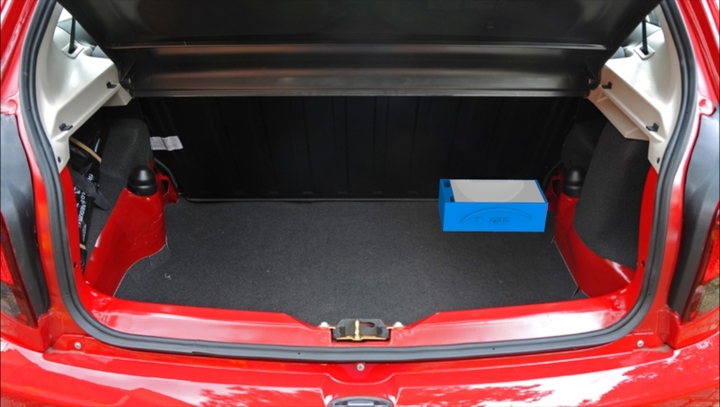
\includegraphics[width=350px, scale=1]{figuras/bagageiro}
  \caption{Localização da caixa protetora no porta-malas}
\label{fig:bagageiro}
\end{figure}

\section{Consumo Energético}
 
A escolha da Bateria foi feita a partir de consultas na Brasal Veículos que informou que a bateria que equipa o Gol G3/G4 1.0 é a bateria Heliar HI50GD
 
\subsection{Bateria HI50GD}

O modelo escolhido apresenta tais especificações:

\begin{itemize}
	\item Ampere Hora (AH): 50 AH
	\item Reserva Cap (min): 75 min
	\item Corrente de partida a frio: 400ª
\end{itemize}

\begin{figure}[h]
  \centering
  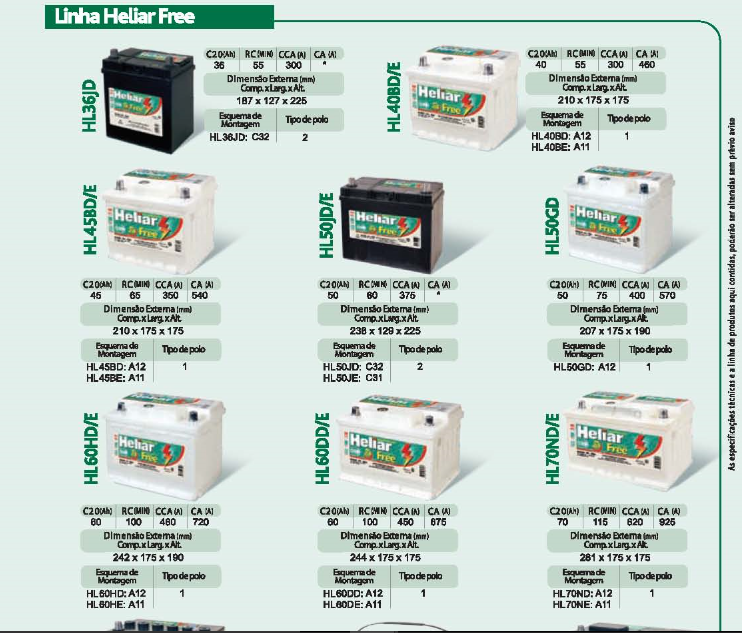
\includegraphics[width=350px, scale=1]{figuras/especificacoes2}
  \caption{Especificações da Bateria Heliar}
\label{fig:especificacoes2}
\end{figure}
	 
\subsection{Ampere Hora}

O parâmetro escolhido para o dimensionamento da bateria foi o Ampere Hora. Ampere Hora é a medida, conferida em laboratório, da capacidade de armazenamento elétrico que a bateria é capaz de proporcionar em descarga, nas partidas e na alimentação do sistema elétrico.

\subsection{Gastos Energéticos de cada componente}

\begin{itemize}

\item{Câmera AWS650}
O sensor anti-colisão AWS650 apresenta uma potência máxima de 3,2W e opera a 24v. Para que possa ser instalado será necessário um conversor de 12v para 24v, devido a bateria do carro ser de 12v. A partir do cálculo de potência, chega-se à
conclusão que a corrente consumida é de 0,1333A.

Pot = U*i;

3,2W = 24v * i

i = 0,133A

\item{Lidar HDL-64E}

O sensor Lidar HDL-64E opera a 15v e 4mA . Sua instalação dependerá de um conversor de 15v para 12v pelo mesmo motivo da câmera. Sua potência é de:

Pot = U*i

Pot = 15v*4A

Pot = 60W

\item{Sensor de Rotação PST 360}

Esse sensor trabalha a 12v com uma corrente de 8,5mA. Na sua instalação não é necessário um conversor, já que, como a bateria, opera a 12v. Apresenta uma potência de:

Pot = U*i

Pot = 12v * 8,5mA

Pot = 0,102W

\item{GPS ME1000RW}

A partir do data sheet a potência máxima do GPS é quando ele atua com 6v e 23mA, portanto, sua potência é de:

Pot = U*i

Pot = 6v * 23mA

Pot = 0,138W

\item{Radar  ARS-30x}
O consumo do radar a 14 volts é de 7W. Como outros equipamentos do projeto é necessário um conversor de 14v para 12v.

\item{Interface TFT054A}
A partir de informações do seu data sheet sabe-se que o consumo da interface
TFT054A é de 79,2mW = 0,08W

\item{Transponder}
O consumo do Transponder, a partir de suas especificações é de 10W.

\item{Processador AM335x}
Sobre o ARM: ele funciona com 90mA no máximo, ou seja, se são 69 portas então são 1,3mA em uma porta GPIO. Opera a uma tensão de 3.3v. Para sua instalação também será necessário um conversor para 12v. Sua potência é de:

Pot = U*i

Pot = 3,3v * 90mA

Pot = 0,3W

\item{GPS A220-A}
Verificando-se o data sheet desse GPS tem-se os seguintes valores: tensão de 6v e corrente de 23mA. Assim como outros equipamentos também será necessário a instalação de um conversor para que possa operar em 12v.

Pot = U*i

Pot = 6v * 23mA

Pot = 0,138W

\item{Laser Nano Series}
O Laser Nano Series opera a uma tensão de 3v com uma corrente de 500mA, portanto sua potência é de:

Pot = U*i

Pot = 3v*500mA

Pot = 1,5W

\end{itemize}

$ Consumo total = 3,2W + 60W + 0,102W + 0,138W + 7w + 0,08W + 10W +0,3 +0,138W + 1,5W = 82,458 $

Sendo assim, temos que a corrente utilizada pelo sistema é de:
	$ Pot = U * i $

	$ 82,458W = 12v * i $

	$ i = 6,87A $

\section{Autonomia da bateria}
 
A bateria tem uma capacidade de 50A em uma hora, portanto terá uma duração de 436,68min para o sistema. Porém a bateria tem a função de alimentar não só o CIAC como também outros componentes do carro como a farol, alarme e etc. Sendo assim, a partir de pesquisas, temos que o consumo médio do Gol é de 0,043A.

\begin{figure}[h]
  \centering
  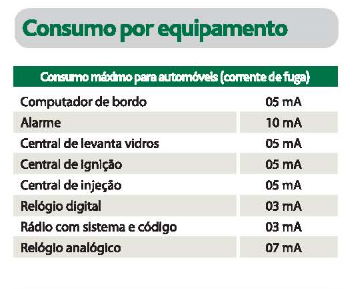
\includegraphics[width=350px, scale=1]{figuras/consumo_equip}
  \caption{Consumo por equipamento de um veículo}
\label{fig:consumo_equip}
\end{figure}

Portanto, o cálculo envolvendo todos os componentes é dado por:
50A são consumidos em uma hora e 6,913A serão consumidos em 433, 96 min (7,23h) caso o alternador pare de funcionar.

\section{Gerência de Custos}

Sabe-se que todo projeto envolve um custo que deve ser orçamentado, estimado e controlado. Infelizmente, em metodologias ágeis como o Scrum não há ferramentas nem técnicas em gestão de custos. Esse aspecto não é nem considerado como parte do cenário. Para isso o melhor a se fazer é a mescla de abordagens de ferramentas e técnicas de gerenciamento de custos.

Os processos de gerência de custo de um projeto incluem:

\begin{itemize}
	\item Planejamento da gestão de custos: avaliar quais recursos e a quantidade aproximada de cada um dentro do projeto;
	\item Estimativa de custo: desenvolver uma aproximação dos gastos com os recursos necessários para execução do projeto;
	\item Orçamento de Custo: agregar os custos estimados de atividades ou de pacotes individuais de trabalho para estabelecer uma base de custo;
	\item Controle de Custo: influenciar nos fatores que geram uma variação de custo e controlar as mudanças de orçamento do projeto.
\end{itemize}

A fim de englobar ao máximo esses 4 itens o Modelo ABC será usado juntamente com análises e comparações de preços dos produtos
 
O CIAC funcionará com 10 dispositivos e são eles:

\begin{table}[]
\centering
\caption{Tabela de custo dos Equipamentos}
\label{custo_equip}
\begin{tabular}{ll}
	Componentes & Custo (R\$) \\ 
	GPS ME1000RW & R\$ 98,94\\
	GPS A220-A & R\$ 25,00\\
	Lidar HDL64E & R\$ 276.750,00\\
	Radar ARS-30X & R\$ 13.840,00\\
	Sensor de Rotação PST360 & R\$ 234,39\\
	Câmera AWS650 & R\$ 3.701,28\\
	Laser Nano Series & R\$ 258,91\\
	Interface TFT054A & R\$ 36,53\\
	Microprocessador & R\$ 40,14\\
	Transponder & R\$ 2.700,00\\
	Caixa de acoplamento & R\$ 30,00
\end{tabular}
\end{table}

O Custo dos equipamentos totaliza R\$ 297.685,42.

Além deste custo, tem-se o custo dos recursos necessários para realizar o projeto. Esse custo foi calculado de acordo com o Método ABC que é um método de custeio que está baseado nas atividades que a empresa efetua no processo de fabricação de seus produtos e ou serviços. Fornece um método para o tratamento dos custos indiretos, através da análise das atividades, dos seus geradores de custos, e dos utilizadores. A idéia básica é atribuir primeiramente os custos às atividades e posteriormente atribuir custos das atividades aos produtos. Sendo assim, primeiramente faz-se o rastreamento dos custos que cada atividade causou, atribuindo-lhes estes custos, e posteriormente verificam-se como os portadores finais de custos consumiram serviços das atividades, atribuindo-lhes os custos definidos. Conforme Eller (2000, p. 82), "o Custeio Baseado em Atividades parte da premissa de que as diversas atividades desenvolvidas geram custos e que os produtos consomem essas atividades".  

\begin{figure}[h]
  \centering
  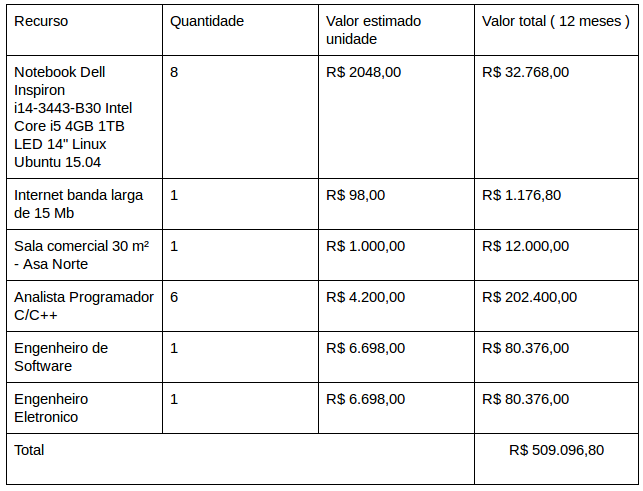
\includegraphics[width=350px, scale=1]{figuras/custo_soft}
  \caption{Custos do desenvolvimento do software}
\label{fig:custo_soft}
\end{figure}

\subsection{Justificativas}

A maneira inicial idealizada para desenvolver as estimativas de custo do software era por analogia,  ou seja, as estimativas de tamanho do projeto seriam baseadas em estimativas já desenvolvidas em projetos similares. Entretanto, além de existirem poucos projetos semelhantes, as empresas detentoras dos direitos autorais de tais projetos, não disponibilizam, separadamente, os custos de fabricação e o tempo de desenvolvimento do software.

Como nao existem softwares livres ou pagos semelhantes, que atendam aos requisitos exigidos pelo projeto, não há como realizar a aquisição de um sistema pronto que possa ser adaptado, ou utilizado em partes no projeto. Portanto, faz-se necessário contratar uma empresa especializada em softwares de sistemas embarcados para construir o sistema desejado. Além disso, por se tratar de um sistema crítico, não é viável a utilização de módulos prontos, os quais podem ocasionar erros durante sua execução e durante a integração de diferentes módulos.

Para contemplar o plano de custo da produção da solução de software do projeto, elaborou-se estimativas do custo da equipe, equipamentos, local de trabalho e tempo necessário, para o seu desenvolvimento.

A estimativa do tempo foi feita com base na dificuldade observada no  pseudo algoritmo do software, na sua arquitetura e no risco de falhas ou erros durante a utilização, com isto foram estipulados 12 meses para o término de seu desenvolvimento. Esse tempo pode ser aumentado de acordo com a necessidade da equipe da empresa escolhida para desenvolvê-lo.

Para cada dia adicionado ao tempo inicial estipulado para o desenvolvimento do software, deverá ser acrescido um valor de R\$ 1984,70 ao seu custo total. Este preço foi obtido através do cálculo da soma do valor mensal de cada um dos gastos do software dividido por 20 dias, visto que os desenvolvedores trabalham 5 dias na semana, 8 horas por dia.

Espera-se que a equipe escolhida tenha um número fixo de 8 pessoas, sendo dividida da seguinte forma:

\begin{itemize}
\item 1 engenheiro de software;
\item 1 engenheiro eletrônico;
\item 6 programadores.
\end{itemize}

Sabe-se que o PMBOK não limita o número de pessoas presentes na equipe, enquanto no Scrum, as equipes podem variar de 3 a 9 membros, não contabilizando o Scrum Master e o Product Owner. Por esse motivo, para não restringir a metodologia a ser adotada pela empresa responsável pelo desenvolvimento do software, foi definido que a equipe de desenvolvimento teria 8 membros.

O custo salarial escolhido para os engenheiros envolvidos no projeto foi retirado do Portal CREA-SP, levando-se em consideração que eles devem trabalhar 8h:00 diárias. Já o salário dos desenvolvedores foi escolhido com base na tabela de salários do site Trainning (Education Services), na linha referente aos analistas programadores C/C++.
